\documentclass[a4paper, 12pt, oneside]{article}

%On peut changer "oneside" en "twoside" si onn sait que le résultat sera recto-verso.
%Cela influence les marges (pas ici car elles sont identiques à droite et à gauche)
%%A faire : première image, gere le wrap (diminuer l'intro ?)
%Fairer gaffe cohérence (ex: dewwar et 2 )
%%=============== PACKAGE PERSO
	
\usepackage[table]{xcolor}	
\definecolor{lightgray}{gray}{0.9}

\DeclareUnicodeCharacter{2212}{-}
\usepackage{graphicx}
\graphicspath{{images/}}
\usepackage{caption}
\usepackage{subcaption}
\usepackage{float} % pour mieux gerer les figures
\usepackage{wrapfig}
\usepackage{pdfpages} %ajouter des pdf en page
\usepackage{chemformula} %pour les molécules
\usepackage{xurl}%url trop long
\usepackage{booktabs} %tableau
\newcolumntype{L}{>{\columncolor{gray!20}}l}

\usepackage[top=2.5cm, bottom=2cm, left=2cm, right=2cm]{geometry}

\usepackage{gensymb}

% quelques symboles mathematiques en plus
\usepackage{amsmath}

% le tout en langue francaise
\usepackage[english]{babel}

% onn peut ecrire directement les charactères avec l'accent
\usepackage[T1]{fontenc}

% a utiliser sur Linux/Windows
%\usepackage[latin1]{inputenc}

% a utiliser avec UTF8
\usepackage[utf8]{inputenc}
%Très utiles pour les groupes mixtes mac/PC. Un fichier texte enregistré sous codage UTF-8 est lisible dans les deux environnement.
%Plus de problème de caractères accentués et spéciaux qui ne s'affichent pas

% a utiliser sur le Mac
%\usepackage[applemac]{inputenc}

% pour l'inclusion de liens dans le document (pdflatex)
\usepackage[colorlinks,bookmarks=false,linkcolor=black,urlcolor=blue, citecolor=black]{hyperref}

\usepackage{units}
\usepackage{verbatim}
\usepackage{verbdef}% http://ctan.org/pkg/verbdef

%Pour changer la taille des titres de section et subsection. Ajoutez manuellement les autres styles si besoin.
\makeatletter
\renewcommand{\section}{\@startsection {section}{1}{\z@}%
             {-3.5ex \@plus -1ex \@minus -.2ex}%
             {2.3ex \@plus.2ex}%
             {\normalfont\normalsize\bfseries}}
\makeatother

\makeatletter
\renewcommand{\subsection}{\@startsection {subsection}{1}{\z@}%
             {-3.5ex \@plus -1ex \@minus -.2ex}%
             {2.3ex \@plus.2ex}%
             {\normalfont\normalsize\bfseries}}
\makeatother





%%%%%%%%%%%%%%%%%%%%%%%%%%%%%%%%%%%%%%%%%%%%%%%%%%%%%%%%%%%%%
%%%%%%  Début du document
%%%%%%%%%%%%%%%%%%%%%%%%%%%%%%%%%%%%%%%%%%%%%%%%%%%%%%%%%%%%%
\begin{document}
\title{\normalsize{Lab Work Report - Group N$^\circ$\\ 11 - XX - NOM TP}}
\date{\normalsize{\today}}
\author{\normalsize{Victor Bonnet} 1\and \normalsize{Mathias Findrihan}}

%De manière à ce que template latex ressemble au mieux au template word, onn empêche latex de créer la page de titre et la créons à la main
%En taille de police 12, la commande \large donne une taille de police 14
%On utilise la commande \sffamily pour créer des caractères sans-serif

\begin{center}
\large\textbf{\sffamily Experiment N$^\circ$ XX - XXXX}\\%
\large\sffamily Group N$^\circ$11: Victor Bonnet, Mathias Findrihan\\%
\large\sffamily \today\qquad NOM PRENOM\\%
\end{center}
%======================================================================================
%===============================Introduction
%======================================================================================
\section{Introduction} %(1/2 page)


Salut, tu peux t'en rendre compte en faisant la somme par composantes des vecteurs $\vec{OA}$ et $\vec{OB}$. En effet on a : 

$$\vec{u}=\vec{OA}+\vec{OB}= R\begin{pmatrix}  \cos\theta\\ \sin\theta\end{pmatrix}+R\begin{pmatrix}  -\cos\theta\\ \sin\theta\end{pmatrix} = R\begin{pmatrix}  \cos\theta-\cos\theta\\ \sin\theta+\sin\theta\end{pmatrix}=R\begin{pmatrix} 0\\2\sin\theta\end{pmatrix}$$

De la même manière, tu trouves le bon résultat pour $\vec{v}$

\begin{figure}[h!]
    \centering
    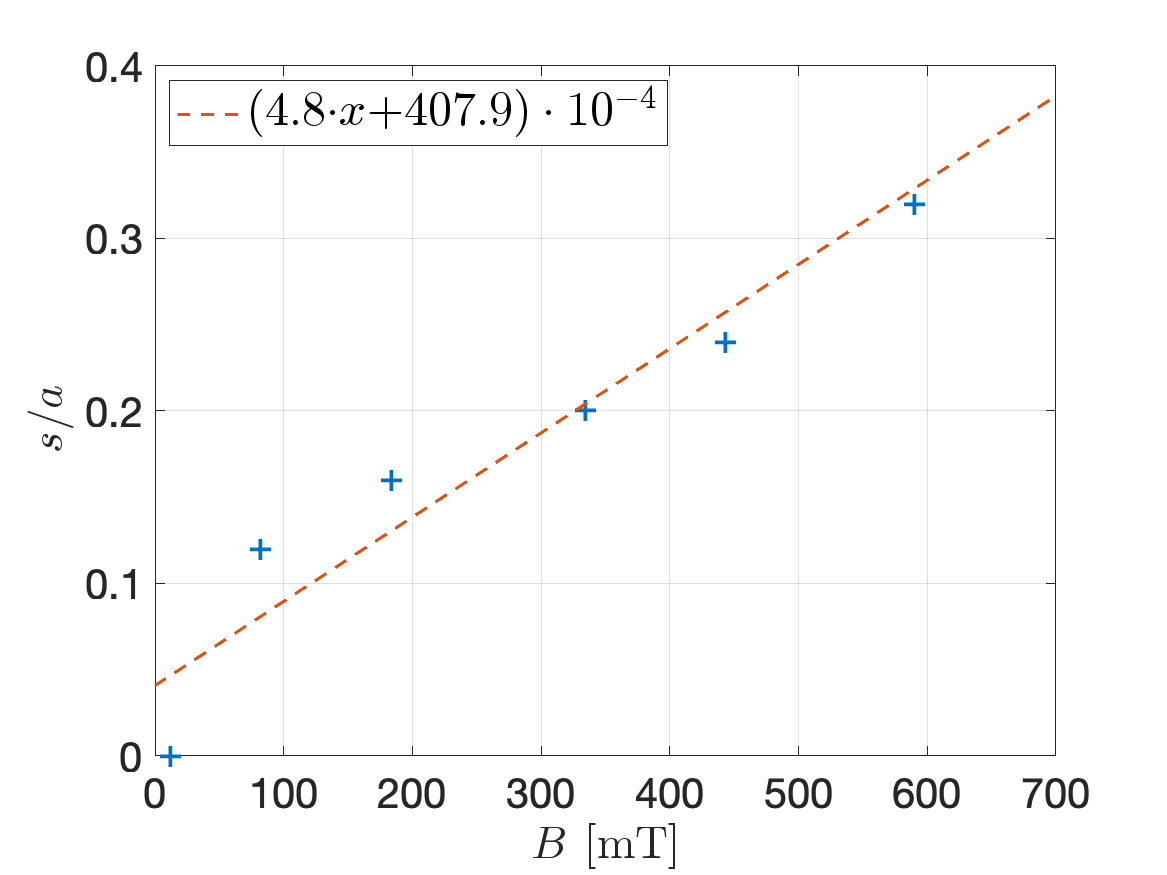
\includegraphics[width=\linewidth]{02_Magneton_T.png}
    \caption{Titre de l'image}
\end{figure}
%======================================================================================
%=================================Démarche
%======================================================================================
\section{Theory \& experimental approach} %(1 page)

%======================================================================================
%=================================RESULTATS
%======================================================================================
\section{Results}%(3-4 pages)

%======================================================================================
%=================================DISCUSSION
%======================================================================================
\section{Discussion}%(1 page)

%======================================================================================
%=================================CONCLUSION
%======================================================================================
\section{Conclusion}%(1/2 page) 




 \pagebreak

%#######################################################################################
%=========================================Bibliographie
%#######################################################################################

\begin{thebibliography}{99}

\end{thebibliography}


%#######################################################################################
%=========================================Annexe
%#######################################################################################
\section{Appendix}
\label{sec:Annexe}

\end{document}

To do : 
